% !TEX TS-program = pdflatex
% !TEX encoding = UTF-8 Unicode

	\documentclass[11pt]{article}                                                    % use larger type; default would be 10pt
\usepackage[utf8]{inputenc}                                                     % set input encoding (not needed with XeLaTeX)

%%% PAGE DIMENSIONS ------------------------------------------------------------
\usepackage[top=0.8in, left=1in, right=1in, bottom=0.8in]{geometry}             % to change the page dimensions
\geometry{a4paper}                                                              % or letterpaper (US) or a5paper or....
\usepackage[parfill]{parskip}                                                   % Activate to begin paragraphs with an empty line rather than an indent

%%% HEADERS & FOOTERS ----------------------------------------------------------
\usepackage{fancyhdr}                                                           % This should be set AFTER setting up the page geometry
\pagestyle{fancy}                                                               % options: empty , plain , fancy
\renewcommand{\headrulewidth}{0pt}                                              % customise the layout...
\lhead{}\chead{}\rhead{}
\lfoot{}\cfoot{page \thepage}\rfoot{}

%%% SECTION TITLE APPEARANCE ---------------------------------------------------
\usepackage{sectsty}
\allsectionsfont{\sffamily\mdseries\upshape}                                    % (See the fntguide.pdf for font help)

%%% PACKAGES -------------------------------------------------------------------
\usepackage[font=small,labelfont=bf,textfont=it]{caption}                       % stylize captions
\usepackage{graphicx}                                                           % support the \includegraphics command and options
\usepackage{booktabs}                                                           % for much better looking tables
\usepackage{array}                                                              % for better arrays (eg matrices) in maths
\usepackage{paralist}                                                           % very flexible & customisable lists (eg. enumerate/itemize, etc.)
\usepackage{verbatim}                                                           % adds environment for commenting out blocks of text & for better verbatim
\usepackage{subfig}                                                             % make it possible to include more than one captioned figure/table in a single float
\usepackage{mathtools}                                                          % for math environments like align
\usepackage{amssymb}                                                            % for symbols like \therefore
\usepackage{verbatim}                                                           % for including text as appears, verbatim
\usepackage{listings}                                                           % for including external files as text, eg code
\usepackage{color}                                                              % for coloring of files and images
\usepackage{overpic}                                                            % for adding annotations to pictures
	\usepackage{siunitx}
	\usepackage{multirow}

%%% EQUATIONS ------------------------------------------------------------------
\numberwithin{equation}{section}                                                % Number equations by section (change for different levels)
	\DeclareSIUnit[number-unit-product = {}]\pixel{\text{pix}}
	\DeclareSIUnit[number-unit-product = {}]\ADU{\text{ADU}}
	\DeclareSIUnit[number-unit-product = {}]\electron{\text{e}^{-{}}}

%% BIBIOGRAPHY ------------------------------------------------------------------
\usepackage{cite}

%%% ToC (table of contents) APPEARANCE -----------------------------------------
%\usepackage[nottoc,notlof,notlot]{tocbibind}                                   % Put the bibliography in the ToC
%\usepackage[titles,subfigure]{tocloft}                                         % Alter the style of the Table of Contents
%\renewcommand{\cftsecfont}{\rmfamily\mdseries\upshape}
%\renewcommand{\cftsecpagefont}{\rmfamily\mdseries\upshape}                     % No bold!

%%% PDF LINKS AND STYLE --------------------------------------------------------
\usepackage[unicode=true,
    bookmarks=true,bookmarksnumbered=true,bookmarksopen=true,
    bookmarksopenlevel=2, breaklinks=false,pdfborder={0 0 0},backref=false,
    colorlinks=false] {hyperref}                                                % for links in pdf file, no colors
\hypersetup{pdftitle={Cosmic Re-ionisation},
    pdfauthor={Extragalactic Astrophysics and Cosmology Group Studies}}			% set name of document and author here

%%% END Article customizations

%%% Include TIKZ images directly into document ---------------------------------
\usepackage[svgnames]{xcolor}
\usepackage{tikz}
\usetikzlibrary{decorations.markings}
\usetikzlibrary{shapes.geometric}

\newif\iffinal                                                                  % introduce a switch for draft vs. final document
\finaltrue                                                                      % use this to compile the final document
\usepackage{tikz}

\iffinal
    \newcommand{\inputTikZ}[1]{%
        \input{#1}%
    }
\else
    \newcommand{\inputTikZ}[1]{%
        \beginpgfgraphicnamed{#1-external}%
        \input{#1}%
        \endpgfgraphicnamed%
    }
\fi

%%% Include svg images directly in document (requires Inkscape) ----------------
\newcommand{\executeiffilenewer}[3]{%
    \ifnum\pdfstrcmp{\pdffilemoddate{#1}}%
        {\pdffilemoddate{#2}}>0%
        {\immediate\write18{#3}}
    \fi
}
\newcommand{\includesvg}[1]{%
    \executeiffilenewer{#1.svg}{#1.pdf}%
    {inkscape -z -D --file=#1.svg --export-pdf=#1.pdf --export-latex}%
    \input{#1.pdf_tex}%
}

%%% NEW COMMANDS ---------------------------------------------------------------
\renewcommand{\d}{\,\mathrm{d}}                                                 % for integrals
\newcommand{\dx}[2]{\frac{\textrm{d} #1}{\textrm{d} #2}}                        % for derivatives
\newcommand{\dd}[2]{\frac{\textrm{d}^2 #1}{\textrm{d} #2^2}}                    % for double derivatives
\newcommand{\pd}[2]{\frac{\partial #1}{\partial #2}}                            % for partial derivatives
\newcommand{\pdd}[2]{\frac{\partial^2 #1}{\partial #2^2}}                       % for double partial derivatives
\newcommand{\e}[1]{\text{e}^{#1}}                                               % for exponentials
\newcommand{\code}[1]{\texttt{#1}}                                              % for verbatim code view
\newcommand{\inter}[1]{\shortintertext{#1}}                                     % shorter version of intertext
\newcommand{\under}[1]{\underline{#1}}                                          % for vectors etc.

\let\vaccent=\v                                                                 % rename builtin command \v{} to \vaccent{}
\newcommand{\uv}[1]{\ensuremath{\hat{#1}}}                                      % for unit vector
\newcommand{\abs}[1]{\left| #1 \right|}                                         % for absolute value
\newcommand{\avg}[1]{\left< #1 \right>}                                         % for average
\let\underdot=\d                                                                % rename builtin command \d{} to \underdot{}
\newcommand{\ket}[1]{\left| #1 \right>}                                         % for Dirac bras
\newcommand{\bra}[1]{\left< #1 \right|}                                         % for Dirac kets
\newcommand{\braket}[2]{\left< #1 \vphantom{#2} \right|
    \left. #2 \vphantom{#1} \right>}                                            % for Dirac brackets
\newcommand{\matrixel}[3]{\left< #1 \vphantom{#2#3} \right|
    #2 \left| #3 \vphantom{#1#2} \right>}                                       % for Dirac matrix elements
\newcommand{\grad}[1]{\nabla #1}                                                % for gradient
\let\divsymb=\div                                                               % rename builtin command \div to \divsymb
\renewcommand{\div}[1]{\nabla \cdot #1}                                         % for divergence
\newcommand{\curl}[1]{\nabla \times #1}                                         % for curl
\let\baraccent=\=                                                               % rename builtin command \= to \baraccent
\renewcommand{\=}[1]{\stackrel{#1}{=}}                                          % for putting numbers above =


%*******************************************************************************
%******************************** END HEADER ***********************************
%*******************************************************************************

\begin{document}
%!TEX root = mainfile.tex
\begin{titlepage}
  \begin{center}
    \vspace*{\fill}

    \centering
    
\includegraphics[scale=1.0]{Logo.pdf}
    \vfill

    \hrule
    {\LARGE\bf Extragalactic Astrophysics and Cosmology\\Cosmic Reionization \\[0.4cm]}
    \hrule

    \vfill
    \large
    School of Physics and Astronomy\\
    University of Birmingham

    \vfill
    { Joe Baumber,
    	James Bryant,
    	Lewis Clegg,
    	Bethany Johnson,
    	Andrew King,
    	Owen McConnell,
    	Catherine McDonald,
    	Michael O'Neill,
    	Jonathan Shepley,
    	Dorothy Stonell,
    	Rahim Topadar,
    	Josh Wainwright\\}
    \vfill

    \vfill
    \textit{Supervisors:} Graham Smith, Alistair Sanderson, Melissa Gillone \\
    		\vfill
    \textit{Date:} March 2013
    \vfill
    \vfill

    \begin{abstract}
        This study deduces that reionization began at a redshift of $z=17.82$ and ended at a redshift of $z=7\pm 1.8$. This is calculated by directly applying the dynamics of star formation and the ionization rate of neutral hydrogen in the Intergalactic Medium. A photometry strategy consisting of 3 multi-band surveys is proposed in order to observe Lyman Break Galaxies across redshifts 6--17. The surveys will locate $100.5\pm37.0$, $138.7\pm 100.6$, $358.1\pm 158.6$ galaxies in redshift ranges 6--8.5, 8.5--10 and 10--17 respectively. These surveys will be completed by the James Webb Space Telescope and Euclid which are planned for launch in the coming decade. A follow up spectroscopy survey will be used to confirm the redshift and properties of 24, 4 and 48 galaxies in these 3 surveys respectively. The spectroscopy will be carried out using James Webb Space Telescope and a combination of single and multi-slit spectroscopy. It is shown that the use of known gravitational lenses, located between redshift 0.5--0.7, is very beneficial for discovering high redshift candidates as it can increase the depth of surveys by up to 3 magnitudes.
    \end{abstract}


  \end{center}
\end{titlepage}

%\thispagestyle{empty}
%\vspace*{\fill}
%\noindent
%\begin{tabular}{ll}
%\end{tabular}

%\cleardoublepage
%\cleardoublepage

\newpage
\tableofcontents
\newpage
\part{General Theory} % (fold)
	\label{prt:general_theory}

% part general_theory (end)
\newpage
\part{Predictions} % (fold)
	\label{prt:predictions}
	%!TEX root = mainfile.tex

\section{Predictions Group} % (fold)
\label{sec:predictions_group}
	In order for those attempting to observe high redshift galaxies to propose a detailed experimental plan, it is important to know how many galaxies one is expecting to observe within a certain volume of the sky. This is the fundamental purpose of the predictions sub-group; to be able to compute this quantity with the depth of the surveyed volume corresponding directly to redshift. In order to do this, a computer program is required to efficiently calculate this number as a function of redshift, field of view and apparent magnitude enabling those observing to make an informed prediction of the telescope one would need and the observing time required to make definitive observation of such elusive galaxies.

	This section of the project was structured chronologically as follows:
	\begin{itemize}
		\item Research how early galaxies are professionally predicted.
		\item Find a general Schechter function in terms of luminosity and/or magnitude.
		\item Mathematically process this function to ensure it is consistent with the units used by those carrying out the observations.
		\item Build a computer program to automate the process of calculating the number of galaxies from the Schechter function.
		\item Find plausible starting parameters to use in primary program.
		\item Collate parameter data from published papers.
		\item Determine parameter evolution with time.
		\item Plot these results to produce a visual description of how these parameters affect the outcome.
		\item Give expected number of galaxies to the observers.
		\item Refine technique with the inclusion of more advanced adaptations.
	\end{itemize}

	In addition to running a program to calculate the total number of galaxies, there is also a separate program to determine the redshifts at which re-ionization began and ended to be included when calculating the number of galaxies in the main code.

	The beginning of re-ionization has been determined by equating the star formation rate density with the critical star formation rate density required for matter to collapse into galaxies (see section..OWEN). The end of re-ionization occurs when the photons produced in star formation have completely ionized the IGM and hence required direct application of star formation rate densities also. This will be covered in more detail in section~\ref{sec:lower_redshift_limit_on_re-ionization}.

% section predictions_group (end)

	%!TEX root = mainfile.tex

\subsection{Assumptions Made} % (fold)
\label{sub:assumptions_made}
    The mathematical model that will be used in our program is limited by certain assumptions about the universe that we are working in. Some of these are generally held to be true and are accepted widely in the scientific community, others are due to the constraints of what we can mathematically program and the observational data available from previous studies. A major assumption that we are making throughout our work on re-ionisation concerns the type of universe that we exist in. This includes the relative densities of matter with respect to radiation and dark energy, as well as the geometry of the whole universe. 

% subsection assumptions_made (end)

\subsection{Parameter Values} % (fold)
\label{sub:parameter_values}

    It will be assumed that the universe has a curvature of zero, in other words, that the universe is flat. This has been shown before and is generally held to be true, ``we now know that the universe is flat with only a 0.4\% margin of error''\cite{nasa_uni_shape}. This means that we do not need to take into account any of the effects of observing objects near the beginning of the universe when it might have had different properties.

    A second assumption that will be maintained through our calculations concerns the values of the matter, curvature and dark energy constants, $\Omega_M$, $\Omega_k$ and $\Omega_{\Lambda}$ respectively. We will assume that we are living in a matter dominated universe and that these parameters are related to the value of the Hubble parameter by equation~\ref{eq:hubble_parameter}\cite{hubble_parameter_astro_journal},
    \begin{align}
        H^2(z) &= H_0^2\left( \Omega_M {(1+z)}^3 + \Omega_k {(1+z)}^4 + \Omega_{\Lambda} \right) \label{eq:hubble_parameter}\\
        \intertext{where}
        \Omega_k &= 1- \Omega_M - \Omega_{\Lambda}
    \end{align}
    We will use values of $\Omega_M=0.27$ and $\Omega_{\Lambda}=0.728\pm0.015$, in accordance with the $\Lambda$CDM model\cite{WMAP_Observations_Cosmological_Interpretation}.

    There are also a number of parameters in the Schechter function that must be specified. In order to find suitable values to use, we collected data from a number of different sources covering several studies. All of the studies that have been performed in the past concer galaxies at lower redshifts than we are expecting to examine. To get an estimate for the value of each of the parameters at higher redshift, the values found were plotted and the fit expropolated to cover the era nessessary. Since some of the fits demonstrate that these parameters are not constant with time, their evolution shall be incorporated into the calculations.

    The values in the Schechter function that we have determined fits for are $\alpha$, $M^{*}$ and $\phi^{*}$. The data collected for each of these fits is shown in appendix~\ref{app:parameter_fit_data}.
    
% subsection parameter_values (end)

% part predictions (end)
\newpage
\part{Observations} % (fold)
	\label{prt:observations_}
	%!TEX root = mainfile.tex

\section{The Hubble Space Telescope} % (fold)
\label{sec:the_hubble_space_telescope}

	\subsection{Mission Launch} % (fold)
	\label{ssub:mission_launch}
		On April 24th 1990 NASA’s Space Shuttle Discovery launched the world’s first space-based optical telescope; The Hubble Space Telescope (HST), named in honour of American astronomer Edwin P. Hubble. Edwin Hubble’s greatest contribution to astronomy was the Hubble Law which states that galaxies are receding from us at a speed directly proportional to their distance from us. This showed that our universe is expanding, a notion which underpins modern cosmological thinking. The telescope sits in a low-Earth orbit, as shown in figure~\ref{fig:hubble_space_telescope}, at an altitude of 569 kilometres completing one orbit of the Earth every 97\,minutes\cite{Hubsite_1}.
		\begin{figure}[ht]
			\centering
			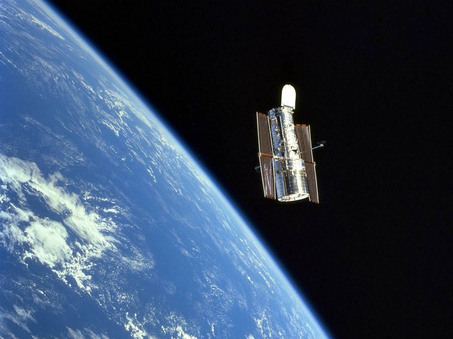
\includegraphics[width=0.5\textwidth]{../Images/Hubble_Space_Telescope.jpg}
			\caption{Photograph of HST orbiting the Earth.\label{fig:hubble_space_telescope}}
		\end{figure}

		The HST was designed to provide clear and deep views of distant galaxies and stars and most of the planets in our solar system. Hubble's domain extends from the ultraviolet through the visible and into the near-infrared\cite{NASA_1}.
	% subsection mission_launch (end)

	\subsection{Achievements to Date} % (fold)
	\label{ssub:achievements_to_date}
		The HST has provided unprecedented detail in images of star formation allowing astronomers to see the jets and disks present during the birth of new stars. It has also been able to study the atmospheric composition of extra-solar planets and take the first visible light picture of a planet outside our solar system; Fomalhaut b\cite{Hubsite_3}.

		Many EoR galaxies and candidate galaxies have been identified using HST data. In December 1995 the HST was pointed at what was believed to be a fairly empty and uninteresting patch of sky; 342 separate exposures were taken over 10 consecutive days and formed an image called the Hubble Deep Field (HDF)\cite{ESA_2}. The image contains around 3,000 objects of which the vast majority are galaxies, with a few local stars in the foreground. The HDF is one of the most iconic images of the 20th century, and it has since been cited in over 800 scientific papers.

		In 2004 its successor was revealed, the Hubble Ultra Deep Field (UDF); a million-second exposure in a 200\si{\arcsecond}$\times$200\si{\arcsecond} area of sky containing \num{10000} galaxies stretching back 13\,billion years\cite{Hubsite_2}. This exposure utilised the recently installed Advanced Camera for Surveys (ACS), seen in figure~\ref{fig:HUDF}. This survey was further refined in September 2012 in the Hubble eXtreme Deep Field (XDF) which utilised the recently installed WFC3 camera as well as combining over \num{2000} separate exposures from different sources\cite{ESA_2}.
		\begin{figure}[ht]
			\centering
			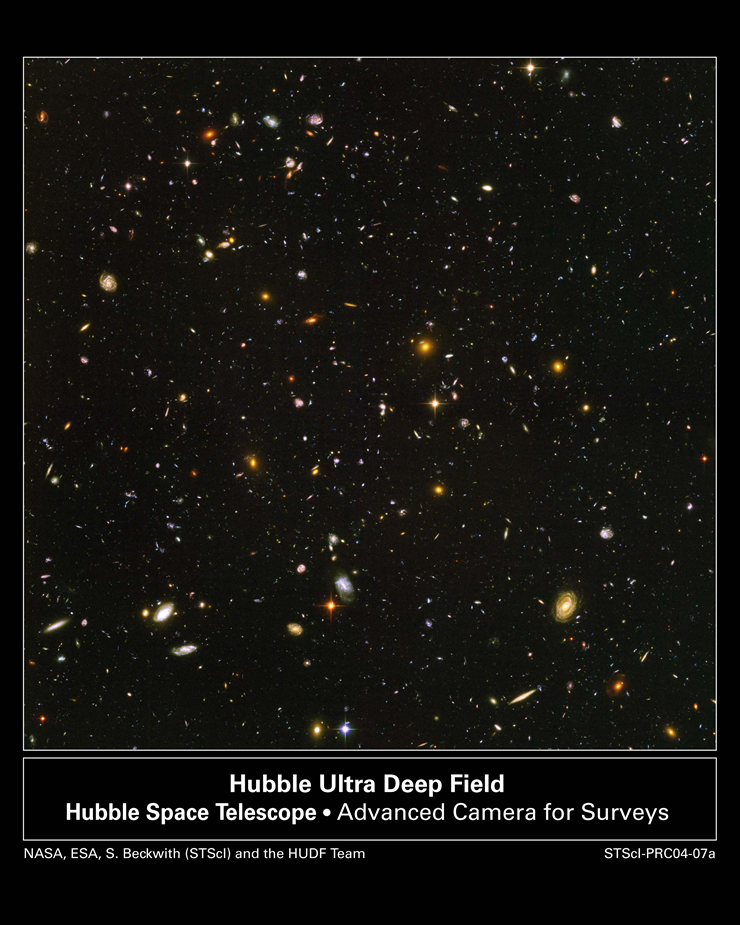
\includegraphics[width=0.8\textwidth]{../Images/HUDF.png}
			\caption{The HUbble Ultra Deep Field.\label{fig:HUDF}}
		\end{figure}

		Using data from the HUDF, object UDFj-39546284 was identified. In a paper by Bouwens et al, published in 2012, their best fit places it at a redshift of $11.8\pm0.3$\cite{Bouwens2012}. This would classify it as the oldest object ever observed. The exact nature of the object is not known but it is believed to be a mini-galaxy. Confirmation will require spectroscopic analysis, which is likely to be carried out by the James Webb Space Telescope. This observation demonstrates both the achievements and limits of the current technology.
	% subsection achievements_to_date (end)

	\subsection{Operation} % (fold)
	\label{ssub:operation}
		The HST is operated remotely from the earth, it has 4 antennae which can send and receive signals from the Flight Operations Team at Goddard Space Flight Centre in Greenbelt, Maryland via the Tracking and Data Relay Satellite system. For communication to be possible HST must have a direct line of sight to at least one of these 5 satellites.

		The HST is powered using 2 arrays of solar panels each capable of converting the Sun’s rays into \num{2800} watts of electricity. The arrays are able to store the electricity in batteries allowing the HST to remain active while in the Earth’s shadow (approximately 36\,minutes out of every 97\,minute orbit).

		Orbiting the Earth subjects the HST to extreme conditions due to the effect of zero gravity and the variation in temperature (up to around \SI{40}{\kelvin}) during each orbit. The optical system is held together using a skeleton (truss) constructed from Graphite epoxy. Graphite epoxy, commonly found in racquets and golf clubs is a stiff and lightweight material able to resist expansion and contraction due to temperature changes\cite{Hubsite_4}.
	% subsection operation (end)

	\subsection{Performance and Optical Telescope Array} % (fold)
	\label{ssub:performance_and_optical_telescope_array}
		The HST is constructed using a Ritchey-Chretien Cassegrain design; this allows high-performance over a wide field of view. The incoming light enters a tube with baffles removing any unwanted stray light, as shown in figure~\ref{fig:HST_optical_diagram} below. The light is then collected by the concave Primary mirror and reflected towards the smaller convex Secondary mirror. This light is then reflected back through a hole in the centre of the Primary mirror where it is focused onto a small area to be picked up by the instruments\cite{Hubsite_5}.
		\begin{figure}[ht]
			\centering
			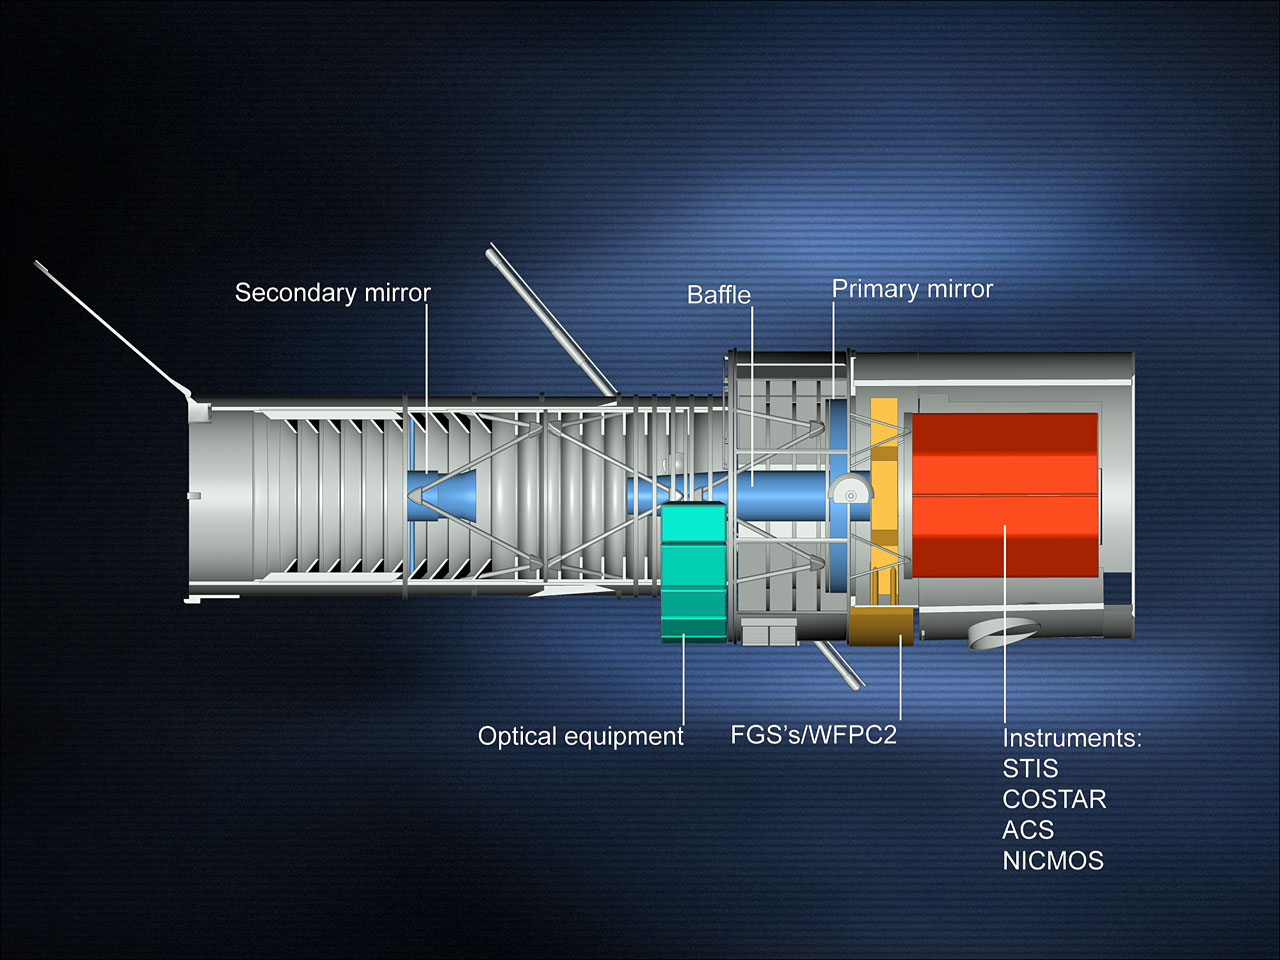
\includegraphics[width=0.5\textwidth]{../Images/HST_optical_diagram.jpg}
			\caption{Diagram showing basic systems of HST, note that WFC2 has since been replaced by WFC3.\label{fig:HST_optical_diagram}}
		\end{figure}

		The mirrors have been polished to an accuracy of better than the wavelength of visible light. When the HST was first launched the scientists soon realised that the curve to which the mirrors had been ground was not correct resulting in an error known as spherical aberration which blurred the images. A servicing mission in December 1993 deployed 5 pairs of mirrors which were able to successfully correct the error and allow Hubble to take the images it was intended to\cite{ESA_1}.

		There have been 4 servicing missions sent to the HST with the final mission taking place in May 2009. Over its lifetime the cameras and instruments have undergone many improvements and replacements. The camera currently operating that is of interest to this project is the WFC3/IR camera, installed in 2009. This camera is able to observe in the near-infra-red where we expect to see the Lyman-break galaxies. Table~\ref{tab:HST_technical} shows the key technical data for the HST, amazingly the HST is so precise it is able to lock onto a target at a distance of 1 mile without deviating more than the width of a human hair.
		\begin{table}[ht]
			\begin{center}
				\begin{tabular}{l|l}
					Component	& 	Details \\
					\hline\hline
					Primary Mirror Diameter & \SI{2.4}{\metre} \\ \hline
					Secondary Mirror Diameter & \SI{0.3}{\metre} \\ \hline
					Wavelength range & 800--1700\si{\nano\metre} \\ \hline
					Total Field of View & \SI{123}{\arcsecond}$\times$\SI{136}{\arcsecond} (\SI{16728}{\arcsecond}$^2$) \\ \hline
					Pixel Size & $18\times18$\,\si{\micro\metre} \\ \hline
					Plate Scale & \SI{0.13}{\arcsecond\per\pixel} \\ \hline
					\multirow{3}{*}{Quantum Efficiency} & 77\% at \SI{1000}{\nano\metre}\\
					 & 79\% at \SI{1400}{\nano\metre}\\
					 & 79\% at \SI{1650}{\nano\metre}\\ \hline
					Dark count &  \SI{0.048}{\electron\per\second\per\pixel} \\ \hline
					Readout noise & \SI{12.0}{\electron\per\second\per\pixel} \\ \hline
					Full Well & \SI{77900}{\electron} \\ \hline
					Gain & 2.28--2.47\si{\electron\per\ADU} \\ \hline
					Operating Temperature & \SI{145}{\kelvin} \\ \hline
					FWHM & \SI{0.151}{\arcminute} at \SI{1600}{\nano\metre}
				\end{tabular}
			\end{center}
			\caption{Technical data for HST WFC3/IR camera system\cite{WFC3_IHB}}
		\label{tab:HST_technical}
		\end{table}
	% subsection performance_and_optical_telescope_array (end)

% section the_hubble_space_telescope (end)

% part observations (end)

\newpage
\appendix
\addcontentsline{toc}{section}{Appendix}

\section{Parameter Fit Data} % (fold)
\label{app:parameter_fit_data}

% section paramter_fit_data (end)
\newpage
\bibliographystyle{unsrt}
\bibliography{references}

\end{document}
    
